\documentclass[conference]{IEEEtran}
\usepackage{amsmath,amsfonts}
\usepackage{algorithm, algpseudocode}
\usepackage{array}
\usepackage[caption=false,font=normalsize,labelfont=sf,textfont=sf]{subfig}
\usepackage{textcomp}
\usepackage{stfloats}
\usepackage{url}
\usepackage{verbatim}
\usepackage{graphicx}
\usepackage{cite}

\usepackage{hyperref} % 引用跳转
\usepackage{natbib}

\usepackage{booktabs} % used for table formatting

\hyphenation{op-tical net-works semi-conduc-tor IEEE-Xplore}

% 参考文献字号
\renewcommand{\bibfont}{\fontsize{8pt}{9pt}\selectfont}

\bibliographystyle{unsrt}

\begin{document}


\title{Reinforcement Learning Project 2 Report\\ Lunar Lander}

\author{Xingyan Liu (202264690069@mail.scut.edu.cn), Shiyi Wang (202230055267@mail.scut.edu.cn) \\Wolin Liang (202264690304@mail.scut.edu.cn), Haoming Jia (202264690267@mail.scut.edu.cn) 
\\Instructor: Ou Shiqi
\thanks{Liu Xingyan: Responsible for code programming, results collation and analysis.Wang Shiyi: Focuses on literature research and problem modeling, specifically defining the problem environment.Liang Wolin: Handles the introduction of related work and paper analysis.Jia Haoming: Analyzes the experimental results and their significance.}% <-this % stops a space
\thanks{Manuscript revised November 10, 2024.}}

% The paper headers
\markboth{Group 1 for Reinforcement Learning, Fall~2024}%
{Shell \MakeLowercase{\textit{et al.}}: A Sample Article Using IEEEtran.cls for IEEE Journals}

\maketitle
\section*{Abstract}

% Below is old abstract DONT DELETE!!!
% \textbf{DQN, a model-free reinforcement learning approach, enables high-dimensional control by approximating the action-value function \( Q(s, a) \) and was implemented in the Lunar Lander environment with systematic hyperparameter tuning. We found that an epsilon decay of \( 0.995 \), a discount factor of \( \gamma = 0.99 \), and a learning rate of \( \alpha = 0.0005 \) yielded optimal results, enabling the agent to achieve a stable landing policy.}

%%% NEW ABSTRACT!!!
\par\textbf{This experiment focuses on the lunar landing mission in the OpenAI Gym environment. A variety of methods, including DQN, DDQN, DDPG, PPO, were used to adjust and optimize their parameters. The results show that different algorithms show different advantages and limitations in the lunar landing mission. Among them, DQN and PPO have the best stability.}

\section{Introduction and related work}

% During the Apollo lunar landings, the lunar module went through several key phases. First, the descent engines slowed down, allowing the module to hover above the lunar surface so that the astronauts could choose a suitable landing site. During this time, the attitude control system made fine adjustments through small nozzles to keep it level and aligned with the landing area. Once the landing site was selected, the lunar module slowly descended, and the thrust was gradually reduced to ensure a smooth contact. When it contacted the lunar surface, the shock absorbers on the landing legs absorbed the impact and ensured that the module was stable. These steps ensured that the lunar module landed safely and protected the astronauts and equipment.

In the Apollo program, engineers used a variety of classical control theories and algorithms to adjust the lunar module to achieve a safe landing. These methods include linear control systems\cite{ogata2010modern}, feedback control\cite{franklin2015feedback}, proportional-integral-derivative (PID) control\cite{astrom2010feedback}, state-space methods\cite{kailath1980linear}, Kalman filtering\cite{kalman1960new}, and optimal control theory\cite{kirk2004optimal}.However, these methods are still insufficient in adaptability and still rely heavily on manual operations in actual operations. Therefore, the problem of using reinforcement learning methods to control the landing capsule for soft landing is proposed\cite{brockman2016openai}.

The LunarLander environment in OpenAI Gym presents a complex control problem involving high-dimensional state spaces and requires sophisticated strategies for successful landings. Several algorithms have emerged as particularly effective in tackling this challenge. 

One of the pioneering approaches is the Deep Q-Network (DQN) \cite{mnih2015human}, which combines deep learning with Q-learning to approximate the Q-function using neural networks. DQN has demonstrated success in handling high-dimensional state spaces and complex decision-making tasks, including those presented by the LunarLander environment. 

Variants of DQN, such as Double DQN \cite{van2016deep} and Dueling DQN \cite{wang2016dueling}, have further enhanced performance by addressing overestimation biases and improving learning efficiency. Proximal Policy Optimization (PPO) is another prominent algorithm, favored for its simplicity and robustness \cite{schulman2017proximal}. PPO utilizes a novel approach to policy gradient methods by constraining the policy updates, which results in more stable training processes. Furthermore, Deep Deterministic Policy Gradient (DDPG), typically applied to continuous action spaces, has been successfully adapted to the continuous version of LunarLander (LunarLanderContinuous-v2) \cite{lillicrap2015continuous}.% DDPG's ability to handle continuous control problems makes it particularly suitable for fine-tuning the lander's control mechanisms. 
% The success of these algorithms is largely attributed to their capability to manage high-dimensional state spaces and optimize complex strategies. Numerous open-source projects and tutorials have demonstrated the implementation and tuning of these algorithms within the LunarLander environment, providing valuable resources for further research and development. These contributions highlight the potential of reinforcement learning in solving intricate control problems and pave the way for future advancements in the field.





\section{Problem Definition}

\texttt{LunarLander-v2} is a reinforcement learning environment from OpenAI Gym designed to simulate the problem of landing a spacecraft. The agent's task is to land the spacecraft safely on the ground within a limited time and avoid collisions.% The state space of the environment includes the spacecraft's position, velocity, angle, angular velocity, and whether it is in contact with the ground. The action space includes four possible actions for the spacecraft: left rocket, right rocket, up rocket, and no operation.

% In this problem, the agent's objective is to learn how to select the optimal actions to maximize cumulative rewards. The reward function evaluates based on whether the spacecraft successfully lands, collides, or lands smoothly.

The state space and the action space is shown as follows:

% state space and action space
\begin{table}[!ht]
    \centering
    \caption{Environment State Space and Action Space}
    \begin{tabular}{lll}
    \toprule
    \textbf{Space Type} & \textbf{Physical Symbol} & \textbf{Details} \\
    \midrule
    State Space & \begin{tabular}[t]{@{}l@{}}$\vec{r}$\\
    $\vec{v}$\\
    $\theta$\\
    $\vec{\omega}$\\
    $C$ (Contact status)\end{tabular} & \begin{tabular}[t]{@{}l@{}}Spacecraft's position \\
    Velocity \\
    Angle \\
    Angular velocity \\
    Whether it is in contact with the ground\end{tabular} \\
    \midrule
    Action Space & \begin{tabular}[t]{@{}l@{}}$F_{left}$\\
    $F_{right}$\\
    $F_{up}$\\
    $F_{none}$\end{tabular} & \begin{tabular}[t]{@{}l@{}}Left rocket \\
    Right rocket \\
    Up rocket \\
    No operation\end{tabular} \\
    \bottomrule
    \end{tabular}
\end{table}


\section{Method Selection and Modeling}

In this problem, we selected four reinforcement learning methods to model and solve the task, each leveraging its specific characteristics to handle the challenges posed by the \texttt{LunarLander-v2} environment.

\subsection{DQN (Deep Q-Network)}

DQN is a reinforcement learning method based on Q-learning that uses deep neural networks to approximate the Q-value function, thereby learning an optimal action-value function for each state. The core idea of DQN is to update the Q-function by minimizing the difference between the estimated Q-values and the actual return.

% \subsubsection*{Reason for Selection}
\par \textit{\quad Reason for Selection:}
\begin{itemize}
    \item The action space in the \texttt{LunarLander-v2} environment is discrete, making DQN a good fit for this type of problem. By using deep neural networks to approximate the Q-value function, it can effectively learn an action strategy in complex environments.
    \item DQN can handle high-dimensional state spaces and improve stability through experience replay and target networks, making it well-suited for environments like \texttt{LunarLander-v2}, which contain significant noise and nonlinear relationships.
\end{itemize}

The Q-function for DQN is defined as:
\[
Q(s, a) = \mathbb{E}\left[ R_t + \gamma \cdot \max_{a'} Q(s', a') \right]
\]
where \(s\) is the current state, \(a\) is the action taken, \(R_t\) is the immediate reward, and \(\gamma\) is the discount factor.

\subsection{DDQN (Double Deep Q-Network)}

% DDQN is an improvement over DQN that aims to reduce the overestimation bias found in Q-learning. In DQN, the maximum Q-value operation can sometimes lead to inaccurate action selection. DDQN solves this by introducing two separate Q-networks: one for action selection and another for calculating the target Q-values.
DDQN is an improvement over DQN that aims to reduce the overestimation bias found in Q-learning. DDQN solves this by introducing two separate Q-networks: one for action selection and another for calculating the target Q-values.

% \subsubsection{Reason for Selection}
\par \textit{\quad Reason for Selection:}
\begin{itemize}
    % \item In DQN, maximizing the Q-value can lead to overestimation, especially during action selection, which may result in suboptimal actions. DDQN addresses this issue by using two independent networks, which allows for more accurate estimation of state-action values and reduces instability caused by overestimation.
    \item In DQN, maximizing the Q - value may cause overestimation during action selection, leading to suboptimal actions. DDQN solves this by using two independent networks for more accurate state-action value estimation and reduced instability from overestimation.
    \item Given the relatively complex state and action spaces in the \texttt{LunarLander-v2} environment, DDQN provides a more robust optimization approach, mitigating potential biases in the estimation process.
\end{itemize}

The Double Q-learning objective in DDQN is:
\[
y = r + \gamma Q_{\text{target}}(s', \arg\max_a Q_{\text{policy}}(s', a))
\]
where \( Q_{\text{policy}} \) is the current policy network and \( Q_{\text{target}} \) is the target network.

\subsection{DDPG (Deep Deterministic Policy Gradient)}

% DDPG is an actor-critic-based reinforcement learning algorithm designed for continuous action spaces. DDPG uses an actor network to select actions and a critic network to evaluate the action's value. It uses stochastic gradient ascent to maximize the policy and stochastic gradient descent to optimize the value function.
DDPG is an actor-critic-based reinforcement learning algorithm designed for continuous action spaces. It uses stochastic gradient ascent to maximize the policy and stochastic gradient descent to optimize the value function.

% \subsubsection{Reason for Selection}
\par \textit{\quad Reason for Selection:}
\begin{itemize}
    \item Although the action space in \texttt{LunarLander-v2} is discrete, DDPG performs exceptionally well on high-dimensional, complex control tasks%, particularly in scenarios where continuous control is needed.
    \item DDPG benefits from combining both actor and critic networks, which helps stabilize the learning process and avoid the limitations of value iteration methods.
\end{itemize}

The DDPG update rules are as follows:
\begin{itemize}
    \item \textbf{Actor}: Updates the policy network parameters using policy gradients.
    \item \textbf{Critic}: Updates the value network parameters by minimizing the mean squared error.
\end{itemize}

\subsection{PPO (Proximal Policy Optimization)}

PPO is a policy gradient method designed to optimize the policy function while maintaining stability by limiting the range of policy updates. This method is particularly suitable for high-dimensional continuous spaces.

% \subsubsection{Reason for Selection}
\par \textit{\quad Reason for Selection:}
\begin{itemize}
    \item The main advantage of PPO is its ability to train the policy in a stable manner when dealing with complex continuous action spaces. It ensures that the policy update step does not lead to excessive policy changes, preventing instability.
    \item PPO has been widely used in reinforcement learning tasks, especially in complex control problems like \texttt{LunarLander-v2}, where it balances exploration and exploitation effectively.
\end{itemize}

The objective function for PPO is:
\[
L^{CLIP}(\theta) = \mathbb{E}_t \left[ \min \left( \rho_t(\theta) \hat{A}_t, \text{clip}(\rho_t(\theta), 1-\epsilon, 1+\epsilon) \hat{A}_t \right) \right]
\]
where \(\rho_t(\theta)\) is the ratio of the current policy to the old policy, \(\hat{A}_t\) is the advantage function, and \(\epsilon\) is a small hyperparameter controlling the range of policy updates.





\section{Experiment and Results}
The DQN algorithm is based on off-policy Q-learning and combines function approximation with experience replay and target network stabilization techniques. Specifically, experience replay helps to decorrelate observations, while the use of a target network mitigates the risk of feedback loops during training, thus improving stability.

%%% DDPG Part
Similarly, DDPG is also an off-policy approximation model. It is based on the coordinated operation of the actor and the critic. While estimating the value of actions, it maximizes the value of actions. Meanwhile, it uses the buffer and the soft update method to stabilize the training process.
\begin{algorithm}
\caption{DQN Algorithm for Lunar Lander}
\textbf{Require:} Environment $\mathcal{E}$, learning rate $\alpha$, discount factor $\gamma$, exploration rate $\epsilon$, decay rate, target update frequency $C$ \\
\textbf{Ensure:} Trained Q-network with optimal action-value function

\begin{algorithmic}[0]
% \State Initialize replay memory $D$ with capacity $N$
% \State Initialize primary Q-network $Q$ with weights $\theta$
% \State Initialize target Q-network $\hat{Q}$ with weights $\theta^{-} \leftarrow \theta$
\State Initialize memory $D$ with $N$, primary Q-network $Q$ with weights $\theta$, and target Q-network $\hat{Q}$ with weights $\theta^{-}\leftarrow\theta$

\For{each episode}
    \State Reset environment, get initial state $s_0$
    \While{not done}
        \State Select action $a_t$:
        \[
        a_t = 
        \begin{cases} 
            \text{random action,} & \text{with probability } \epsilon \\ 
            \arg\max_a Q(s_t, a; \theta), & \text{with probability } 1 - \epsilon 
        \end{cases}
        \]
        \State Execute $a_t$, observe reward $r_t$ and next state $s_{t+1}$
        \State Store transition $(s_t, a_t, r_t, s_{t+1})$ in $D$
        

        \If{$D$ has enough samples}
            \State Sample mini-batch $(s_j, a_j, r_j, s_{j+1})$ from $D$
            \State Compute target $y_j$:
            \[
            y_j = 
            \begin{cases} 
                r_j, & \text{if } s_{j+1} \text{ is terminal} \\ 
                r_j + \gamma \max_{a'} \hat{Q}(s_{j+1}, a'; \theta^{-}), & \text{otherwise} 
            \end{cases}
            \]
            \State Update $\theta$ by minimizing $\left( y_j - Q(s_j, a_j; \theta) \right)^2$
        \EndIf
        
        \If{\text{step mod } $C = 0$}
            \State Update target network: $\theta^{-} \leftarrow \theta$
        \EndIf
    \EndWhile
    \State Decay $\epsilon$ according to decay rate

\EndFor

\end{algorithmic}
\end{algorithm}

%

\begin{algorithm}
\caption{DDPG Algorithm}
\textbf{Require:} Environment $\mathcal{E}$, learning rates $\alpha_{\mu}$ and $\alpha_{Q}$, discount factor $\gamma$, buffer capacity $N$, soft update parameter $\tau$, batch size $M$ \\
\textbf{Ensure:} Trained actor and critic networks

\begin{algorithmic}[0]
\State Initialize replay buffer $D$ and networks $\mu$, $\mu'$, $Q$, and $Q'$ with weights $\theta^{\mu}$, $\theta^{\mu'} \leftarrow \theta^{\mu}$, $\theta^{Q}$, $\theta^{Q'} \leftarrow \theta^{Q}$

\For{each episode}
    \State Reset environment, get initial state $s_0$
    \While{not done}
        \State Generate $a_t = \mu(s_t; \theta^{\mu})$, execute $a_t$, observe $r_t$, $s_{t+1}$
        \State Store $(s_t, a_t, r_t, s_{t+1})$ in $D$
        

        \If{$D$ has enough samples}
            \State Sample mini-batch from $D$
            \State Target: $y_j = r_j + \gamma Q'(s_{j+1}, \mu'(s_{j+1}; \theta^{\mu'}))$
            \State Loss: $L(\theta^{Q}) = \frac{1}{M} \sum_j (y_j - Q(s_j, a_j))^2$
            \State Update actor using policy gradient $\nabla_{\theta^{\mu}} J$
        \EndIf
    
        \State Soft update target networks $\theta^{\mu'}$ and $\theta^{Q'}$
    \EndWhile

\EndFor

\end{algorithmic}
\end{algorithm}


        %%% PPO Algorithm
        \begin{algorithm}
            \caption{PPO Algorithm for LunarLander-v2}
            \textbf{Require:} Environment $\mathcal{E}$, learning rate $\alpha$, discount factor $\gamma$, clipping parameter $\epsilon$, entropy coefficient $\beta$, epochs $K$, batch size $M$ \\
            \textbf{Ensure:} Trained Actor and Critic networks
            \begin{algorithmic}%[1]
            \State Initialize Actor and Critic networks with $\theta$ and $\phi$
            \For{each episode}
                \State Reset environment, obtain initial state $s_0$
                \While{not done}
                    \State Predict action distribution $\pi_\theta(s_t)$ with Actor
                    \State Sample action $a_t$, observe reward $r_t$, next state $s_{t+1}$
                    \State Store $(s_t, a_t, r_t, s_{t+1})$ in buffer
                    \State Update $s_t \leftarrow s_{t+1}$
                \EndWhile
                \State Compute advantages and discounted rewards
                \For{$K$ epochs}
                    \State Sample mini-batch from buffer
                    \State Update Actor using PPO clipped loss
                    \State Update Critic with value loss
                \EndFor
            \EndFor
            
            \Function{ppo\_loss}{$y_{\text{true}}$, $y_{\text{pred}}$}
                \State Compute clipped objective and entropy loss
                \State Return total loss
            \EndFunction
            
            \end{algorithmic}
        \end{algorithm}

\begin{table}[h]
    \centering
    \caption{Hyperparameter Values for PPO Training}
    \begin{tabular}{|>{\centering\arraybackslash}m{3.5cm}|>{\centering\arraybackslash}m{1.5cm}|}
        \hline
        \textbf{Hyperparameter} & \textbf{Value} \\
        \hline
        Learning Rate ($\alpha$) & 0.0003 \\
        \hline
        Discount Factor ($\gamma$) & 0.99 \\
        \hline
        Clip Range ($\epsilon$) & 0.2 \\
        \hline
        Entropy Coefficient ($\beta$) & 0.01 \\
        \hline
        GAE Lambda ($\lambda$) & 0.95 \\
        \hline
        Batch Size & 64 \\
        \hline
        Number of Epochs ($K$) & 10 \\
        \hline
        Replay Buffer Size & 100,000 \\
        \hline
    \end{tabular}
    \label{tab:hyperparams}
\end{table}





\subsection{Network Architecture and Hyperparameters}
The neural network used for Q-value approximation has two hidden layers, each with 64 units, and ReLU activation functions. The hyperparameters are selected based on empirical results and prior studies on DQN performance in similar environments. The chosen values are as follows:
	\begin{table}[h]
		\centering
		\caption{Hyperparameter Values for DQN Training}
		\begin{tabular}{|>{\centering\arraybackslash}m{3.5cm}|>{\centering\arraybackslash}m{1.5cm}|}
			\hline
			\textbf{Hyperparameter} & \textbf{Value} \\
			\hline
			Learning Rate ($\alpha$) & 0.001 \\
			\hline
			Discount Factor ($\gamma$) & 0.99 \\
			\hline
			Exploration Rate ($\epsilon$) & 1.0 (initial) \\
			\hline
			Decay Rate & 0.995 \\
			\hline
			Replay Memory Size ($N$) & 100000 \\
			\hline
			Target Update Frequency ($C$) & 1000 steps \\
			\hline
			Batch Size & 64 \\
			\hline
		\end{tabular}
		\label{tab:hyperparams}
	\end{table}

        %%% DDPG Hyper params
        \begin{table}[h]
    	\centering
    	\caption{Hyperparameter Values for DDPG Training}
    	\begin{tabular}{|c|c|}
    		\hline
    		\textbf{Hyperparameter} & \textbf{Value} \\
    		\hline
                Number of Episodes & 1000\\
                \hline
                Buffer Capacity ($N$) & 100000\\
                \hline
                Batch Size ($M$) & 64\\
                \hline
                Discount Factor ($\gamma$) & 0.99\\
                \hline
                Soft Update Parameter ($\tau$) & 0.001\\
                \hline
                Learning Rate of Actor Network ($\alpha_\mu$) & 0.0001\\
                \hline
                Learning Rate of Critic Network ($\alpha_Q$) & 0.001\\
    		\hline
    	\end{tabular}
    	\label{tab:hyperparams}
    \end{table}


\subsection{Results}
The training results show clear progress in the agent’s performance. Figure \ref{fig:mean_scores}, early scores are highly variable and often negative, reflecting the agent's initial struggles. Over time, scores trend upward, frequently exceeding 200, indicating improved skill. Figure \ref{fig:training_scores} confirms this, showing a steady rise in average scores, reflecting the agent's growing consistency. By the end, the agent reaches near-target scores, proving that the DQN, DDQN, DDPG, and PPO algorithm and fine-tuning enabled it to learn an effective landing strategy. 

\begin{figure}[!ht]
    \centering
    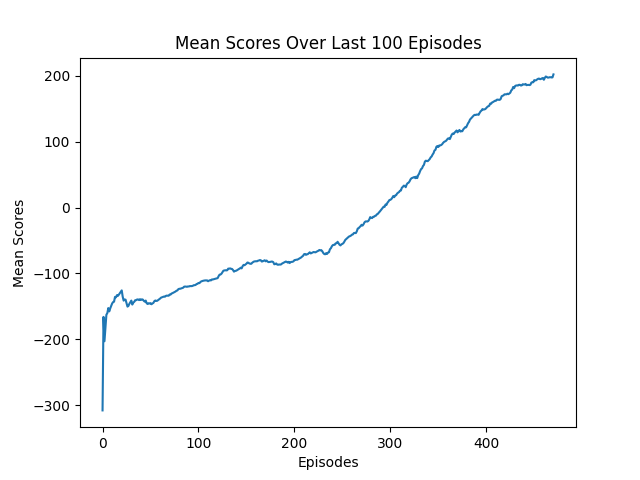
\includegraphics[width=0.8\linewidth]{Figure_2.png}
    \centering
    \caption{Mean Scores over the Last 100 Episodes}
    \label{fig:mean_scores}
\end{figure}

\begin{figure}[!ht]
    \centering
    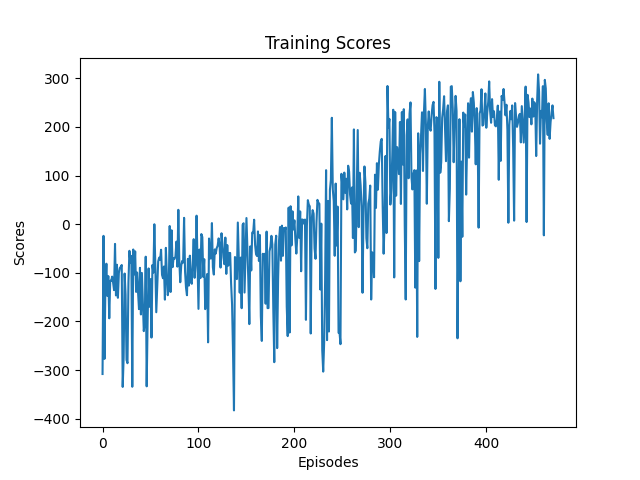
\includegraphics[width=0.8\linewidth]{Figure_1.png}
    \centering
    \caption{Training Scores over Episodes}
    \label{fig:training_scores}
\end{figure}


Additional experiments were performed to assess the impact of different hyperparameters, including epsilon decay, discount factors, and learning rates. The outcomes are presented in Figures \ref{fig:epsilon_decay_over_time}, \ref{fig:gamma_scores}, and \ref{fig:learning_rate_scores}. 

\section{Result Analysis}

In this section, we analyze the experimental results in depth, with a focus on the effects of various hyperparameters such as epsilon decay, discount factor $\gamma$, and learning rate $\alpha$. 

% A
\subsection{Epsilon Decay Over Episodes}
% The analysis in Figure \ref{fig:epsilon_decay_over_time} shows that the discount factor ($\gamma$) strongly affects the agent's stability and performance. Higher values, like $\gamma = 0.99$, lead to more consistent and higher scores, as they help the agent prioritize long-term rewards, which is crucial in complex tasks. Lower values, such as $\gamma = 0.5$, result in greater score variability and lower overall performance, reflecting a short-sighted strategy. Mid-range values show some improvement but lack the stability of the highest discount factor. Thus, a high discount factor proves effective for achieving a stable, high-performing policy.
The analysis in Figure \ref{fig:epsilon_decay_over_time} shows the discount factor ($\gamma$) strongly affects the agent's stability and performance. Higher values (e.g., $\gamma = 0.99$) lead to more consistent and higher scores as they make the agent prioritize long-term rewards, crucial in complex tasks. Lower values (e.g., $\gamma = 0.5$) cause greater score variability and lower performance, reflecting a short-sighted strategy. Mid-range values improve but lack the stability of the highest discount factor. Thus, a high discount factor is effective for a stable, high-performing policy.

\begin{figure}[!ht]
    \centering
    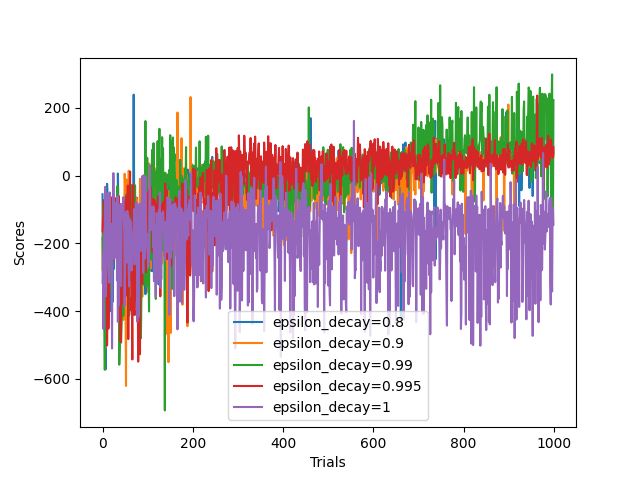
\includegraphics[width=0.8\linewidth]{Figure_4.png}
    \caption{Epsilon Decay Over Time for Different Decay Rates}
    \label{fig:epsilon_decay_over_time}
\end{figure}

\subsection{Impact of Discount Factor $\gamma$}
% The discount factor $\gamma$ determines the extent to which future rewards are valued relative to immediate rewards. A high $\gamma$ value (e.g., 0.99) enables the agent to prioritize long-term rewards, which is essential in the Lunar Lander environment where optimal strategies often involve controlled, gradual maneuvers. Figure \ref{fig:gamma_scores} shows that epsilon decay rate strongly affects the agent’s performance. A slower decay rate (0.995) promotes balanced exploration, leading to higher and more stable scores as training progresses. This gradual shift from exploration to exploitation helps the agent develop a well-rounded policy. Faster decay rates (0.8 and 0.9), however, push the agent to exploit too soon, resulting in lower and more inconsistent scores. Thus, a decay rate of 0.995 appears optimal, providing enough exploration to support stable learning.
The discount factor $\gamma$ determines the value of future rewards relative to immediate ones. A high $\gamma$ (e.g., 0.99) makes the agent prioritize long - term rewards, crucial in the Lunar Lander environment with optimal strategies involving controlled maneuvers. Figure \ref{fig:gamma_scores} shows epsilon decay rate affects performance. A slower decay rate (0.995) promotes balanced exploration, leading to higher and more stable scores during training, helping the agent develop a good policy. Faster decay rates (0.8 and 0.9) make the agent exploit too soon, resulting in lower and inconsistent scores. So, a decay rate of 0.995 is optimal for stable learning.

\begin{figure}[!ht]
    \centering
    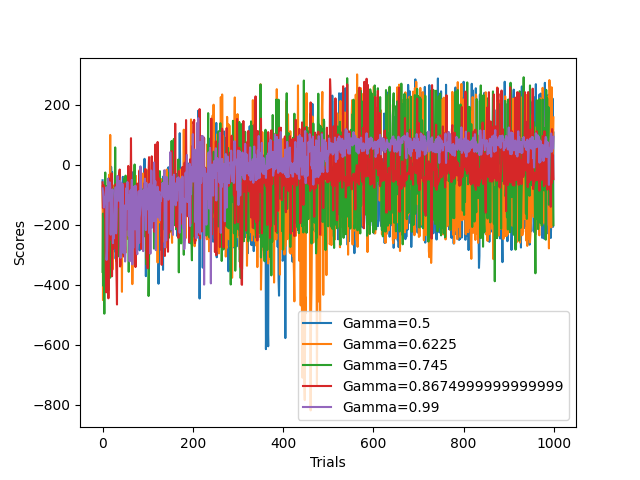
\includegraphics[width=0.8\linewidth]{Figure_6.png}
    \caption{Scores with Different Discount Factors}
    \label{fig:gamma_scores}
\end{figure}

\subsection{Impact of Learning Rate $\alpha$}
% The learning rate $\alpha$ affects the speed and stability of the network's weight updates during training. As shown in Figure \ref{fig:learning_rate_scores}, an optimal learning rate of 0.0005 allowed the agent to converge efficiently while maintaining stability in the training process. Lower learning rates (e.g., $5 \times 10^{-5}$) led to slower convergence, as the updates to the Q-network were too small to capture the underlying dynamics of the environment effectively. On the other hand, excessively high learning rates (e.g., 0.05 or 0.5) introduced instability, with the agent frequently diverging from optimal policies and exhibiting large performance fluctuations. This observation aligns with standard DQN practices, suggesting that moderate learning rates are key to achieving a balanced convergence rate without sacrificing training stability.
The learning rate $\alpha$ impacts the speed and stability of network weight updates during training. As Figure \ref{fig:learning_rate_scores} shows, an optimal rate of 0.0005 enables efficient convergence and stability. Lower rates (e.g., $5\times10^{-5}$) slow convergence as Q-network updates are too small for effective environment dynamics capture. High rates (e.g., 0.05 or 0.5) cause instability, with the agent diverging from optimal policies and having large performance fluctuations, consistent with standard DQN practice where moderate rates are key for balanced convergence without sacrificing stability.

\begin{figure}[!ht]
    \centering
    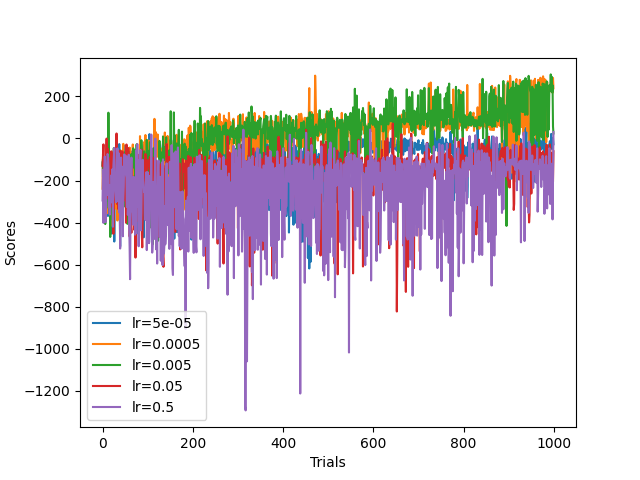
\includegraphics[width=0.8\linewidth]{Figure_7.png}
    \caption{Score Variability for Different Learning Rates}
    \label{fig:learning_rate_scores}
\end{figure}

Figure \ref{fig:epsilon_decay_rates} shows how different epsilon decay rates affect the transition from exploration to exploitation. Faster decay rates, like 0.8, reduce epsilon quickly, pushing the agent into exploitation early. Moderate rates (0.9 and 0.99) offer a more balanced shift. The slowest rate, 0.995, allows prolonged exploration, helping the agent learn a more stable policy. A rate of 1.0, with no decay, keeps the agent in constant exploration, hindering effective learning. Thus, a decay rate of 0.99 best supports a gradual and beneficial transition.

\begin{figure}[h]
    \centering
    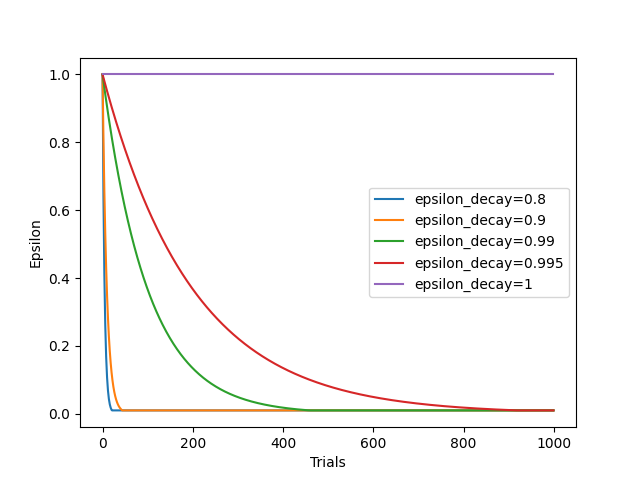
\includegraphics[width=0.8\linewidth]{Figure_5.png}
    \caption{Epsilon Per Training Trial Given Different Epsilon Decay Rates}
    \label{fig:epsilon_decay_rates}
\end{figure}

%%% DDPG Result
\subsection{Impact of Model Selection in DDPG Training}
% In this DDPG experiment, in order to adapt to this task, the team designed three networks with different levels of complexity for the actor and four networks with different levels of complexity for the critic respectively. The networks for the actor are as follows: a pure MLP (Linear), an MLP with LayerNorm (LinearNorm), and a deep network with residual blocks (Residue). The networks for the critic are divided into 1 and 2 according to whether the inputs are entered separately or combined, and are further divided into Linear and Residue according to the complexity of the network. Therefore, the networks for the critic are Linear1, Linear2, Residue1, and Residue2. Thus, there are a total of 12 networks in the experiment. After 12 independent experiments, the results are as Figure 7.
In this DDPG experiment, the team designed 3 actor networks (pure MLP (Linear), MLP with LayerNorm (LinearNorm), deep network with residual blocks (Residue)) and 4 critic networks (Linear1, Linear2, Residue1, Residue2 based on input combination and complexity) for the task. There are 12 networks in total. After 12 independent experiments, the results are as Fig \ref{fig:12Combs}.
\begin{figure}[!ht]
    \centering
    \includegraphics[width=1\linewidth]{12Combs.png}
    \caption{Rewards' and Steps' curves in DDPG Training}
    \label{fig:12Combs}
\end{figure}

\subsection{Experiment Summary for PPO on LunarLander-v2}

The experiment aimed to train a Proximal Policy Optimization (PPO) agent on the \texttt{LunarLander-v2} environment. The graph below shows the agent’s performance over the training cycle, measured by the episode score.

\begin{figure}[h]
    \centering
    \includegraphics[width=0.4\textwidth]{Figure_8.png}
    \caption{Training Performance of PPO on LunarLander-v2}
\end{figure}

\subsection*{Observations}



During training, the agent's score showed significant fluctuations. In the initial phase, the score often dropped into negative values, reflecting difficulty in landing. As training progressed, the score improved, indicating better control and fewer crashes. In the later phase, the score stabilized around positive values, showing that the agent had learned a stable landing strategy, with only minor fluctuations remaining.


\subsection*{Conclusion}
The PPO agent successfully learned to control the lander over time, as indicated by the increasing and stabilizing average score. Despite the variability in individual episode scores, the overall trend shows effective learning and improved performance in the \texttt{LunarLander-v2} environment.

%%%
% \subsection{Insights and Recommendations}
% This analysis reveals key insights into how hyperparameter selection impacts DQN performance in continuous control tasks. A balanced epsilon decay rate, particularly around 0.995, is essential for thorough exploration in complex environments like Lunar Lander. This slower decay prevents premature convergence, allowing the agent to gather a richer set of experiences before prioritizing exploitation. A high discount factor ($\gamma = 0.99$) further supports stable, long-term policy optimization, which is advantageous in tasks requiring foresight. Together, these parameters promote the learning of robust, adaptable strategies.

% Additionally, a moderate learning rate (0.0005) is crucial to achieving stable convergence. This rate effectively balances the speed of learning with stability, allowing the agent to capture environmental dynamics without risking divergence. Overall, the DQN agent effectively learns a policy for the Lunar Lander environment when hyperparameters are carefully tuned. Future work could enhance this approach by integrating advanced techniques, such as Dueling DQN and prioritized experience replay, to improve stability and accelerate learning. Testing the agent across varied scenarios could also provide insights into the generalizability and robustness of the learned policy.
%%%

% \vfill

\bibliographystyle{plain}
\bibliography{references}

\end{document}